\documentclass[tikz,border=6pt]{standalone}
\usepackage[T1]{fontenc}
\usepackage{lmodern}
\usepackage{amsmath,amssymb}
\usetikzlibrary{positioning,arrows.meta,fit,calc}
% Design of koblitz-n83-rankfinder-20261021 (frozen protocol.json and schedule.json). Not a result.
\begin{document}
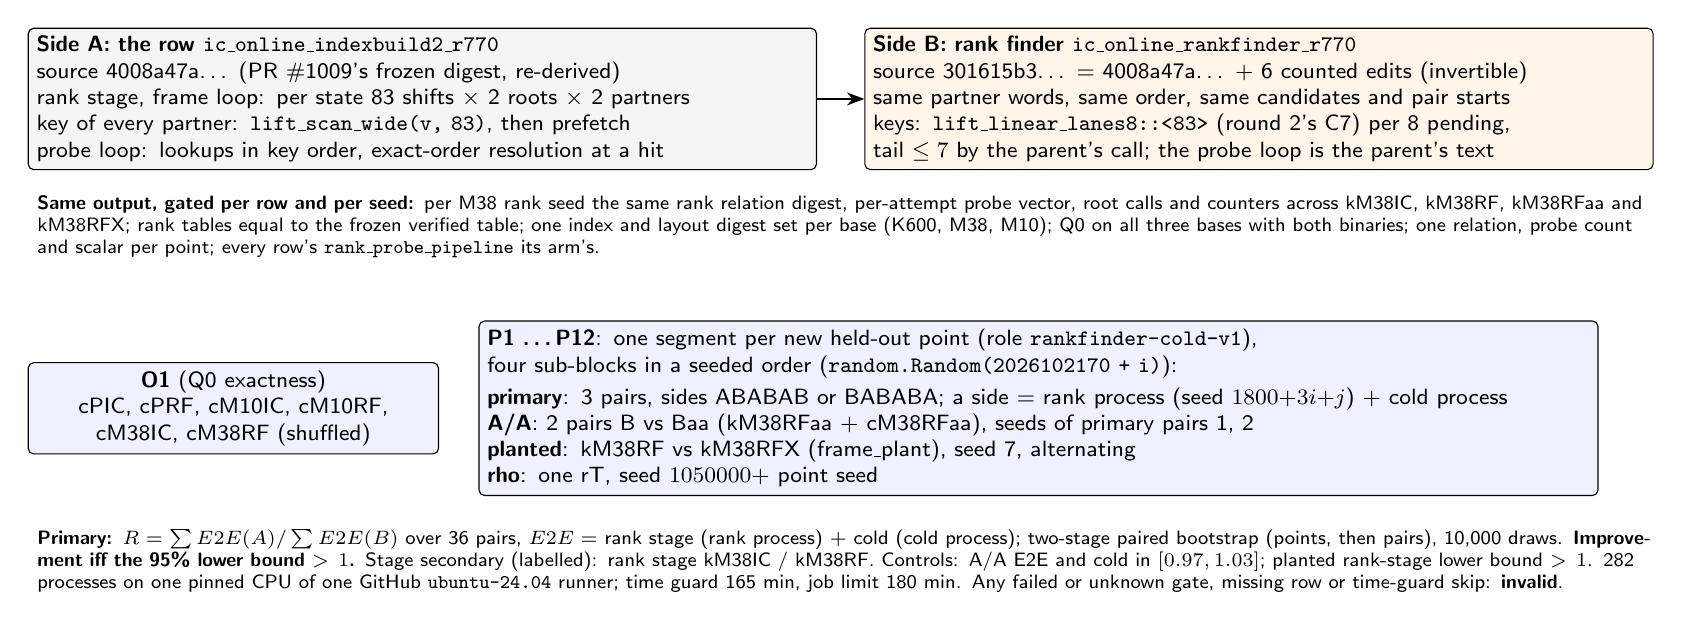
\begin{tikzpicture}[
  font=\sffamily\footnotesize,
  box/.style={draw, rounded corners=2pt, align=center, minimum height=8mm, inner sep=3pt},
  arr/.style={-{Stealth[length=2.2mm]}, thick},
  note/.style={align=left, font=\sffamily\scriptsize}
]
\node[box, fill=gray!8, text width=98mm, align=left] (pa) {\textbf{Side A: the row} \texttt{ic\_online\_indexbuild2\_r770}\\
source 4008a47a\ldots\ (PR \#1009's frozen digest, re-derived)\\
rank stage, frame loop: per state 83 shifts $\times$ 2 roots $\times$ 2 partners\\
key of every partner: \texttt{lift\_scan\_wide(v, 83)}, then prefetch\\
probe loop: lookups in key order, exact-order resolution at a hit};
\node[box, fill=orange!8, text width=98mm, align=left, right=6mm of pa] (pb) {\textbf{Side B: rank finder} \texttt{ic\_online\_rankfinder\_r770}\\
source 301615b3\ldots\ = 4008a47a\ldots\ + 6 counted edits (invertible)\\
same partner words, same order, same candidates and pair starts\\
keys: \texttt{lift\_linear\_lanes8::<83>} (round 2's C7) per 8 pending,\\
tail $\le 7$ by the parent's call; the probe loop is the parent's text};
\draw[arr] (pa.east) -- (pb.west);
\node[note, below=2mm of pa.south west, anchor=north west, text width=205mm] (same) {\textbf{Same output, gated per row and per seed:} per M38 rank seed the same rank relation digest, per-attempt probe vector, root calls and counters across kM38IC, kM38RF, kM38RFaa and kM38RFX; rank tables equal to the frozen verified table; one index and layout digest set per base (K600, M38, M10); Q0 on all three bases with both binaries; one relation, probe count and scalar per point; every row's \texttt{rank\_probe\_pipeline} its arm's.};
% schedule
\node[box, fill=blue!6, text width=50mm, below=12mm of same.south west, anchor=north west] (o1) {\textbf{O1} (Q0 exactness)\\ cPIC, cPRF, cM10IC, cM10RF,\\ cM38IC, cM38RF (shuffled)};
\node[box, fill=blue!6, text width=140mm, align=left, right=5mm of o1] (p) {\textbf{P1 \ldots P12}: one segment per new held-out point (role \texttt{rankfinder-cold-v1}),\\ four sub-blocks in a seeded order (\texttt{random.Random(2026102170 + i)}):\\[2pt]
\textbf{primary}: 3 pairs, sides ABABAB or BABABA; a side = rank process (seed $1800{+}3i{+}j$) + cold process\\
\textbf{A/A}: 2 pairs B vs Baa (kM38RFaa + cM38RFaa), seeds of primary pairs 1, 2\\
\textbf{planted}: kM38RF vs kM38RFX (frame\_plant), seed 7, alternating\\
\textbf{rho}: one rT, seed $1050000 + $ point seed};
\node[note, anchor=north west, text width=205mm] at ($(o1.west |- p.south)+(0,-3mm)$) {\textbf{Primary:} $R=\sum E2E(A)/\sum E2E(B)$ over 36 pairs, $E2E=$ rank stage (rank process) $+$ cold (cold process); two-stage paired bootstrap (points, then pairs), 10{,}000 draws. \textbf{Improvement iff the 95\% lower bound $>1$.} Stage secondary (labelled): rank stage kM38IC / kM38RF. Controls: A/A E2E and cold in $[0.97,1.03]$; planted rank-stage lower bound $>1$. 282 processes on one pinned CPU of one GitHub \texttt{ubuntu-24.04} runner; time guard 165 min, job limit 180 min. Any failed or unknown gate, missing row or time-guard skip: \textbf{invalid}.};
\end{tikzpicture}
\end{document}
